\documentclass[useAMS, usenatbib, a4paper]{mnras}
\pdfsuppresswarningpagegroup=1

\usepackage[spanish,es-minimal,english]{babel}
\usepackage[utf8]{inputenc}
\usepackage{graphicx}
\graphicspath{ {../figs/} }
\usepackage{xcolor}
\usepackage{fixltx2e}
\usepackage{hyperref}
\usepackage{siunitx}
\usepackage{newtxtext}
\usepackage[varg,varvw,smallerops]{newtxmath}
\usepackage{booktabs}
\hypersetup{colorlinks=True, linkcolor=blue!50!black, citecolor=black,
  urlcolor=blue!50!black}
\usepackage{etoolbox}
\robustify\bfseries
\robustify\itshape
\bibliographystyle{mnras}

\sisetup{
  % explicit""+" is useful for velocities
  retain-explicit-plus = true,
  % prefer 10^6 over 1 x 10^6
  retain-unity-mantissa = false,
  % Use x +/- e instead of x(e)  
  separate-uncertainty = true,
  % Make sure to pick up bold font when used in section heading for instance
  detect-weight = true,
}
% A better \ion command that works in more circumstances
\newcommand\ION[2]{#1\,\scalebox{0.9}[0.8]{\uppercase{#2}}}
\newcounter{ionstage}
\renewcommand{\ion}[2]{\setcounter{ionstage}{#2}% 
  \ensuremath{\mathrm{#1\,\scriptstyle\Roman{ionstage}}}}
\newcommand\hii{\ion{H}{2}}
\newcommand\nii{[\ion{N}{2}]}
\newcommand\oiii{[\ion{O}{3}]}


\title{Kinematics of the Turtle Nebula (Will's part)}

\author[Henney]{
  William J. Henney\thanks{w.henney@irya.unam.mx}\\
  \foreignlanguage{spanish}{Instituto de Radioastronomía y
    Astrofísica, Universidad Nacional Autónoma de México, Apartado
    Postal 3-72, 58090 Morelia, Michaoacán, Mexico}
}
% These dates will be filled out by the publisher
\date{Accepted XXX. Received YYY; in original form ZZZ}

% Enter the current year, for the copyright statements etc.
\pubyear{2020}

\begin{document}
\label{firstpage}
\pagerange{\pageref{firstpage}--\pageref{lastpage}}
\maketitle

\begin{abstract}
  Material to be incorporated into the main paper by Teresa.
\end{abstract}
\begin{keywords}
  Atomic physics -- Radiative transfer -- Photodissociation regions
\end{keywords}


\begin{figure}
  \centering
  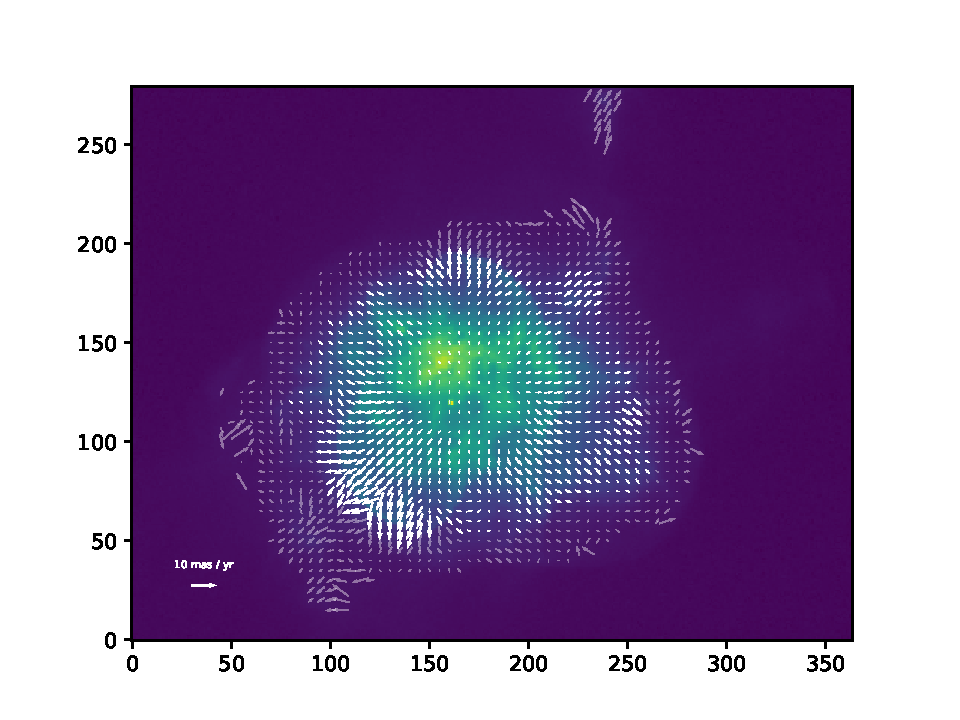
\includegraphics[width=\linewidth]{oiii-propermotions}
  \caption{Proper motions derived from two HST \oiii{} images (F502N
    filter) separated by 10.45 years, using the FLCT algorithm with a
    Gaussian window width of 10~pixels. The key at bottom left shows a
    proper motion of \SI{10}{mas.yr^{-1}}, corresponding to
    \SI{95}{km.s^{-1}} for an assumed distance of \SI{2}{kpc}.}
  \label{fig:proper-motions-oiii}
\end{figure}
\begin{figure}
  \centering
  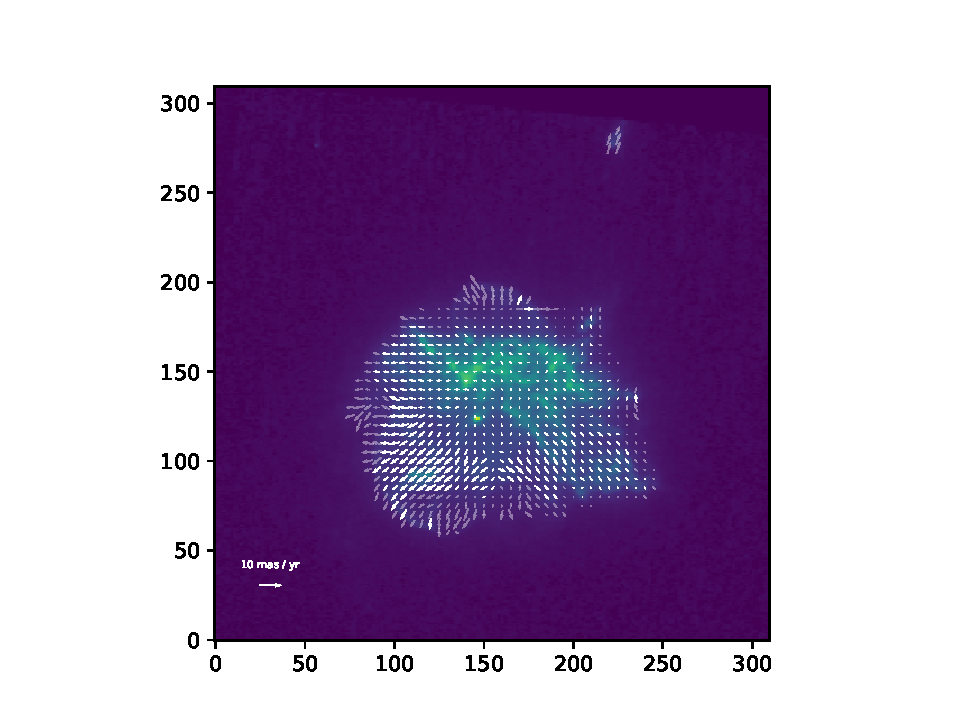
\includegraphics[width=\linewidth]{nii-propermotions}
  \caption{As Fig.~\ref{fig:proper-motions-oiii} but for two HST
    \nii{} images (F658N filter). Note that the field of view is
    cropped slightly smaller than for \oiii{}.}
  \label{fig:proper-motions-nii}
\end{figure}

\begin{figure*}
  \centering
  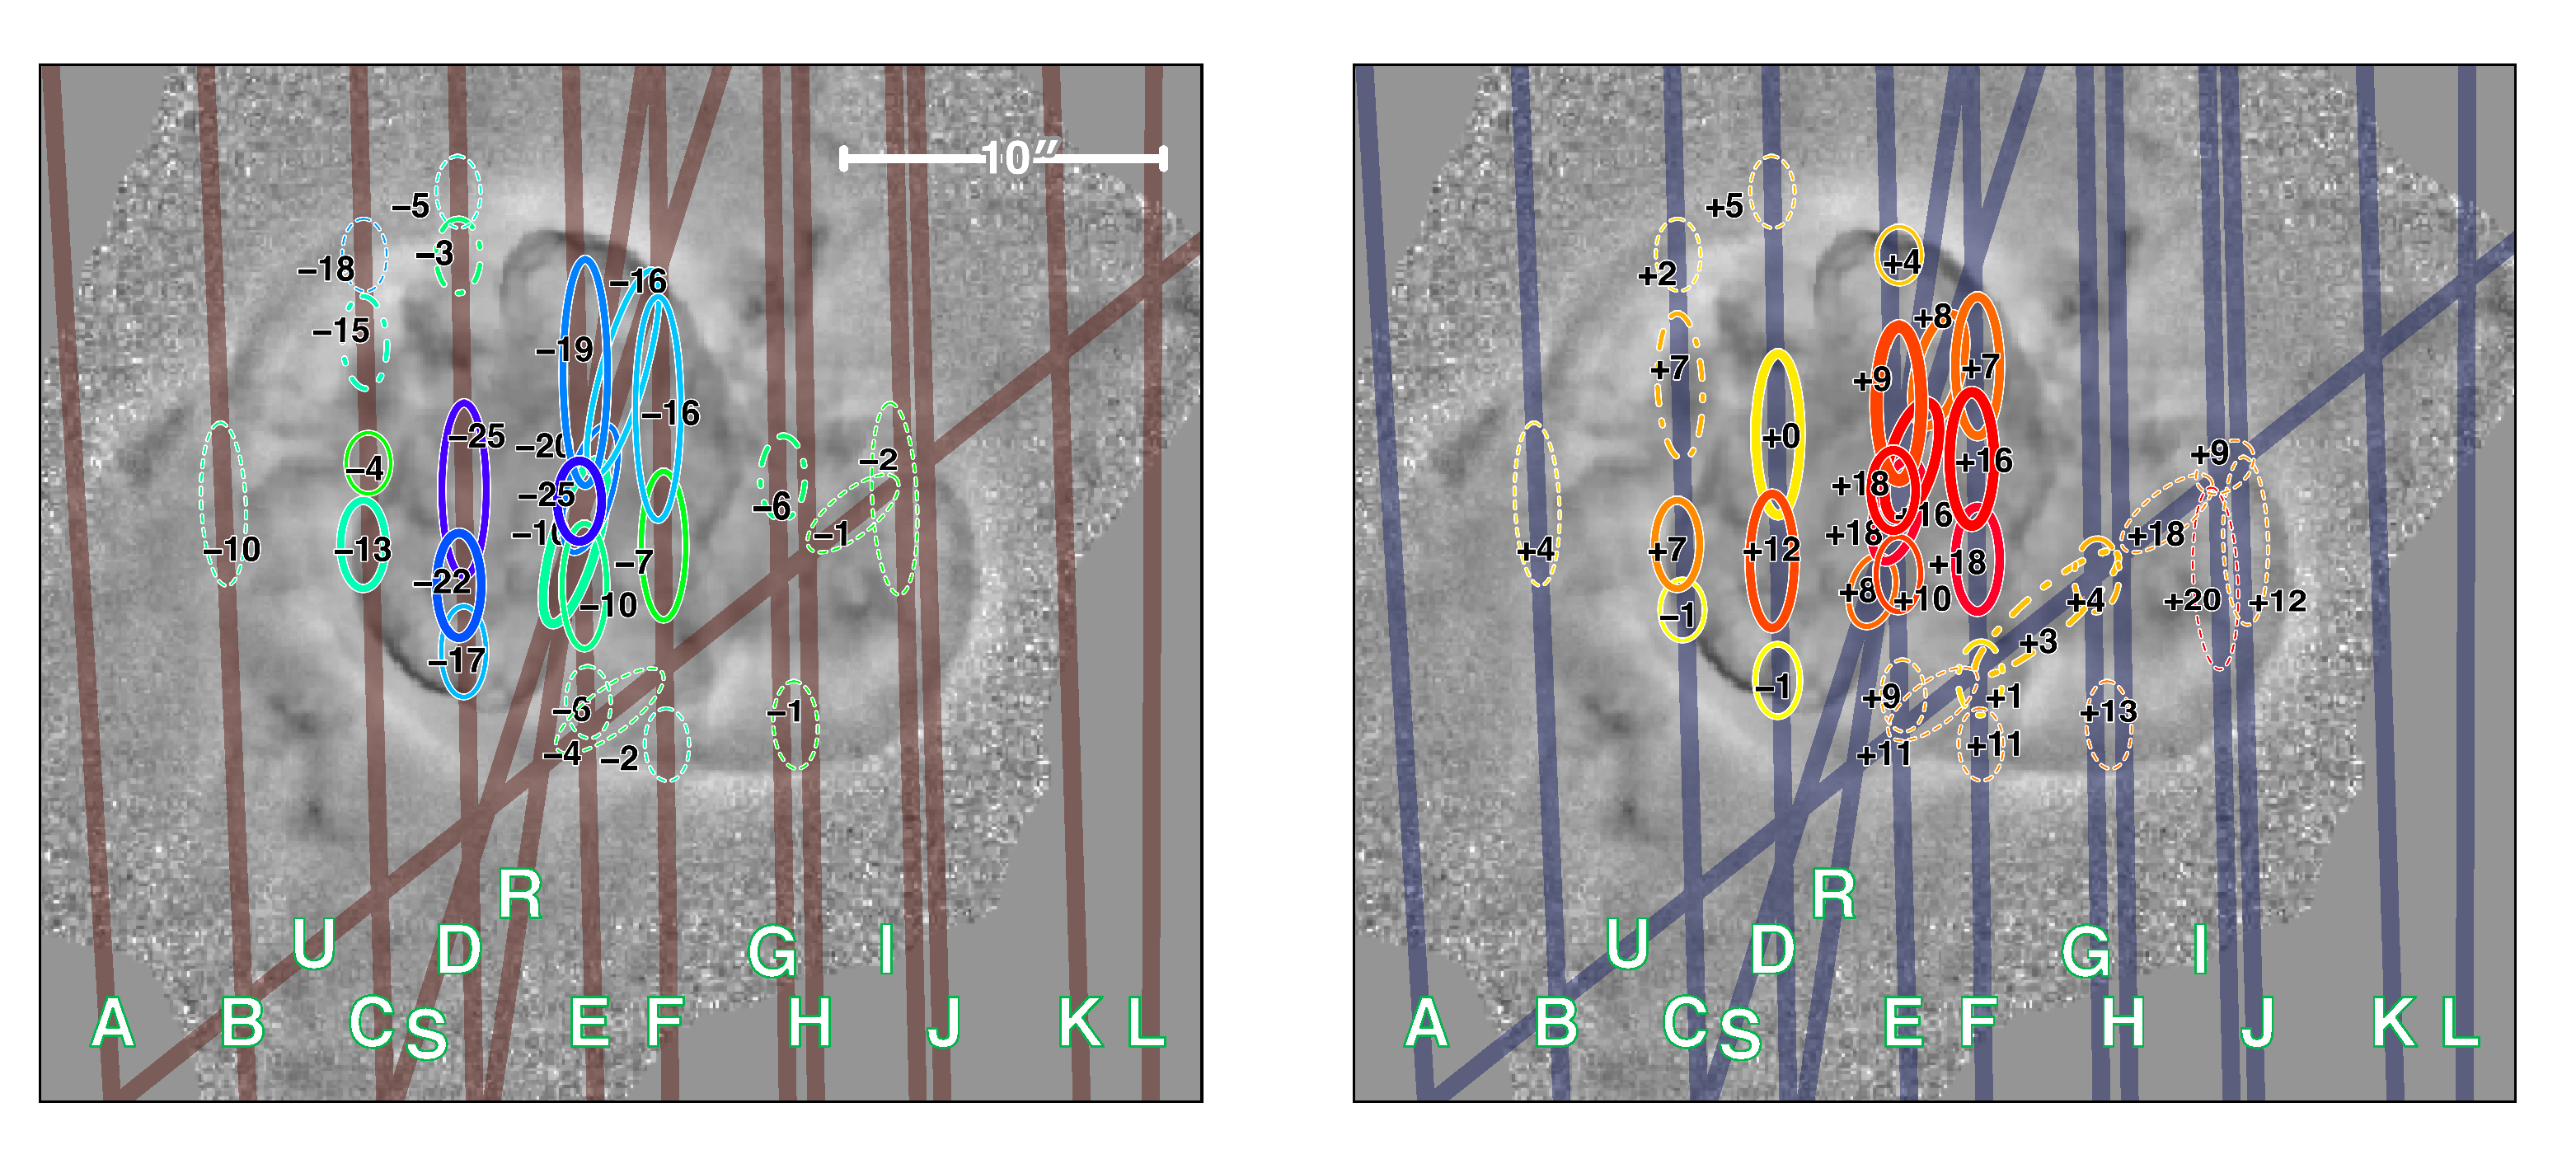
\includegraphics[width=\linewidth]{turtle-peanut-map}
  \caption{
    Velocity features in the high-ionization shells,
    which have been identified in the \oiii{} slits.
    Left panel shows blue-shifted features,
    while right panel shows red-shifted features,
    each labelled with their line-of-sight velocity
    with respect to the nominal systemic velocity of \SI{40}{km.s^{-1}}.
    Solid lines show features in the inner shells,
    dashed lines show features in the intermediate shell,
    and dot-dashed lines show miscellaneous features between the two shells.
    The line width is a qualitative indicator of the brightness of each feature.
  }
  \label{fig:shell-velocity-components}
\end{figure*}

\begin{figure}
  \centering
  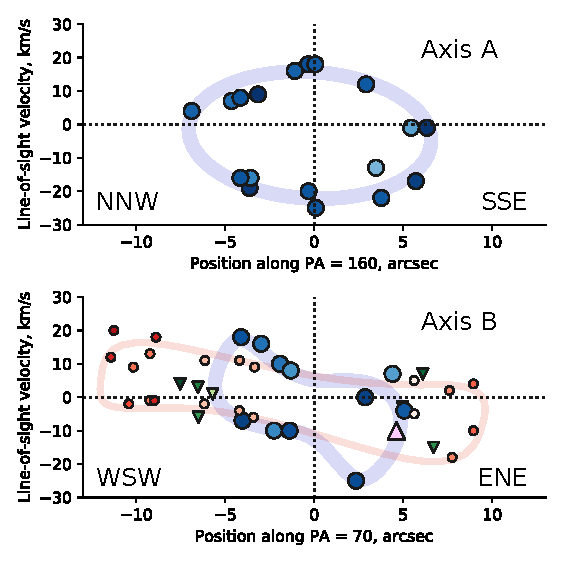
\includegraphics[width=\linewidth]{turtle-shell-velocity-axes-annotated}
  \caption{
    Radial velocity versus position
    for the shell features shown in Fig.~\ref{fig:shell-velocity-components}.
    Results are shown along two axes:
    Axis~A (upper panel) is the apparent major projected axis of the inner shells,
    while Axis~B (lower panel) is perpendicular to this.
    Large blue circles show the inner shell,
    small red circles show the intermediate shell,
    and green triangles show miscellaneous features between the two shells.
    Darker colors indicate features that are closer to each respective axis.
    Colored lines are merely to guide the eye,
    and show possible interpretations of the shell kinematics along the two axes.
  }
  \label{fig:shell-velocity-axes}
\end{figure}


\section{Introduction}
\label{sec:introduction}

\section{Observations and data reduction}
\label{sec:observ-data-reduct}

\section{Longslit spectroscopy}
\label{sec:longsl-spectr}

\newpage
\section{Proper motions}
\label{sec:proper-motions}

Proper motions are calculated from HST WFPC2 imaging at two epochs separated by approximately 10 years,
using the FLCT method \citep{Welsch:2004a, Fisher:2008a}.\footnote{
  We used version 1.07 of FLCT, obtained from \url{http://cgem.ssl.berkeley.edu/cgi-bin/cgem/FLCT/home},
  together with version 1.04 of the Python wrapper pyflct,
  obtained from \url{https://github.com/PyDL/pyflct}.}
Results are shown in Figures~\ref{fig:proper-motions-oiii} and~\ref{fig:proper-motions-nii} for \oiii{} and \nii{}, respectively.
In both cases, the images were remapped to a uniform square pixel grid at the WFC resolution of \SI{0.1}{arcsec.pix^{-1}} before applying the algorithm.
The resultant per-pixel motions between the two epochs are found to be of order \SI{0.5}{pix} (\(\approx \SI{5}{mas.yr^{-1}}\))
and these raw results were then corrected by applying a global shift to force the motion of the central star to be zero.
The systematic error from the global alignment of the two epochs is estimated to be \SI{1.5}{mas.yr^{-1}},
which is expected to dominate the proper motion uncertainties in the brighter parts of the nebula.
In fainter and more featureless regions of the nebula, the proper motions are increasingly affected by random noise,
which can be seen in parts of the lobes in Figure~\ref{fig:proper-motions-oiii}.

The corrected results, as shown in the figures, can be seen to display motions that are predominantly radial from the central star.
To convert the angular motions into transverse velocities, we assume a distance of \SI{2}{kpc},
so that \SI{10}{mas.yr^{-1}} is equivalent to \SI{95}{km.s^{-1}}.
From the \oiii{} images (Fig.~\ref{fig:proper-motions-oiii}),
the fastest plane-of-sky motions are of order \SI{60}{km.s^{-1}},
and are chiefly along the NNW--SSE direction,
including the projected major axis of the inner peanut shell,
the NW~knot, the N~jet, and the end-cap of the S~lobe.
Motions along the perpendicular ENE--WSW direction are typically slower,
of order \SI{30}{km.s^{-1}}.
Note that proper motions are unavailable for the end cap of the N lobe since the second epoch HST image does not cover this region.

The \nii{} images (Fig.~\ref{fig:proper-motions-nii}) show a similar expansion pattern for the features that are visible in both lines.
Remarkably low plane-of-sky velocities of \(\le \SI{15}{km.s^{-1}}\) are seen for the \nii{}-bright knot complexes immediately north and west of the central star. 

\section{Kinematic components from slit spectra}
\label{sec:kinematic-components}

In order to investigate the kinematics of the nebula in detail,
we have measured the velocities of distinct emission components in each slit spectrum
and organized them into broad systems based on their location, morphology and degree of ionization.

\subsection{High-ionization shells}
\label{sec:high-ioniz-shells}

These systems represent the majority of the \oiii{} emission in the core of the nebula
and show a nested elliptical shell morphology.
Figure~\ref{fig:shell-velocity-components} shows the \oiii{} emission components associated with these shells,
as derived from the longslit spectra.
Line-of-sight velocities are given with respect to the nominal systemic velocity (\SI{40}{km.s^{-1}} heliocentric),
separated into negative velocities (left panel) and positive velocities (right panel).
The inner ``peanut'' shells, with a radius of \(5''\) to \(7''\), are the brightest
and are indicated by thick-lined colored ellipses. 
The edge of the more extended intermediate shell, with a radius of \(8''\) to \(12''\), is 10 to 100 times fainter than the inner shells
and is indicated by thinner dashed ellipses.
Additional miscellaneous emission features located in between these shells are indicated by dot-dashed ellipses.
Further features that seem to be associated with the low-ionization knots discussed below in \S~\ref{sec:knot-complexes} are omitted from the figure.


Although the inner shell is irregular in shape,
it shows an apparent elongation along \(\text{PA} \approx \ang{160}\).
The intermediate shell is elongated roughly perpendicular to this, along \(\text{PA} \approx \ang{70}\).
In Figure~\ref{fig:shell-velocity-axes} we plot the velocity of each shell component
against position along each of these axes,
which we denote axis~A and axis~B.  
Each component was assigned to only one axis (A or B), according to its location,
but this assignment is unavoidably subjective for components near the center,
where the two axes cross.

Along axis~A a closed velocity ellipse can be seen for the inner shells,
with a maximum splitting of \(\pm \SI{22}{km.s^{-1}}\) close to the central star
and velocities close to zero at either end (\(\pm 7''\)).
The pattern is not entirely symmetric,
with a slight gradient of \(\pm \SI{3}{km.s^{-1}}\) along the length,
in which the more negative velocities are at the SSE end.
The centroid of the ellipse is also shifted by \(\SI{-3.5}{km.s^{-1}}\)
with respect to the systemic velocity.

Along axis~B,
which is the apparent minor axis of the inner shells (\(\pm 5''\)),
the ellipse is distorted and the gradient is much more pronounced:
\(\pm \SI{11}{km.s^{-1}}\),
with the more negative velocities at the ENE end
(large blue circle symbols in lower panel of Fig.~\ref{fig:shell-velocity-axes}).
Velocity splitting of \(\pm \SI{9}{km.s^{-1}}\) is seen near both ends,
but it is not clear from the \oiii{} spectra if the ends are closed or open,
since none of the \oiii{} slits are aligned with this axis.
However, one of the \nii{} slits (slit~W) is indeed oriented close to axis~B and,
although the shells emit only weakly in \nii{},
the distorted ellipse is clearly closed at the ENE end
(large pink triangle symbol in Fig.~\ref{fig:shell-velocity-axes}).
The situation is not so clear at the WSW end
since any \nii{} emission from the shell is swamped by brighter emission from the knot complexes.
However, the evidence from \textit{HST} imaging suggests that the shell is closed in this direction also.

The intermediate shell along axis~B repeats a similar kinematic pattern to the inner shell,
but at larger radii.
It is represented by dashed ellipses in Figure~\ref{fig:shell-velocity-components} and small red circle symbols in Figure~\ref{fig:shell-velocity-axes}.
The gradient (\(\pm \SI{9}{km.s^{-1}}\)) and splitting (\(\pm \SI{8}{km.s^{-1}}\))
are both marginally smaller than for the inner shell.
Note that, unlike the inner shells, the intermediate shell is markedly lop-sided,
extending \(12''\) to the WSW, but only \(10''\) to the ENE.

The miscellaneous high-ionization components lie outside the inner shells
and show a spoke-like morphology on the \textit{HST} images.
It is represented by dot-dashed ellipses in Figure~\ref{fig:shell-velocity-components} and small green triangle symbols in Figure~\ref{fig:shell-velocity-axes}.
They do not show any marked kinematic pattern,
but are broadly compatible with the velocities of nearby portions of the intermediate shell. 

\subsection{Low-ionization knot complexes}
\label{sec:knot-complexes}

\begin{figure*}
  \centering
  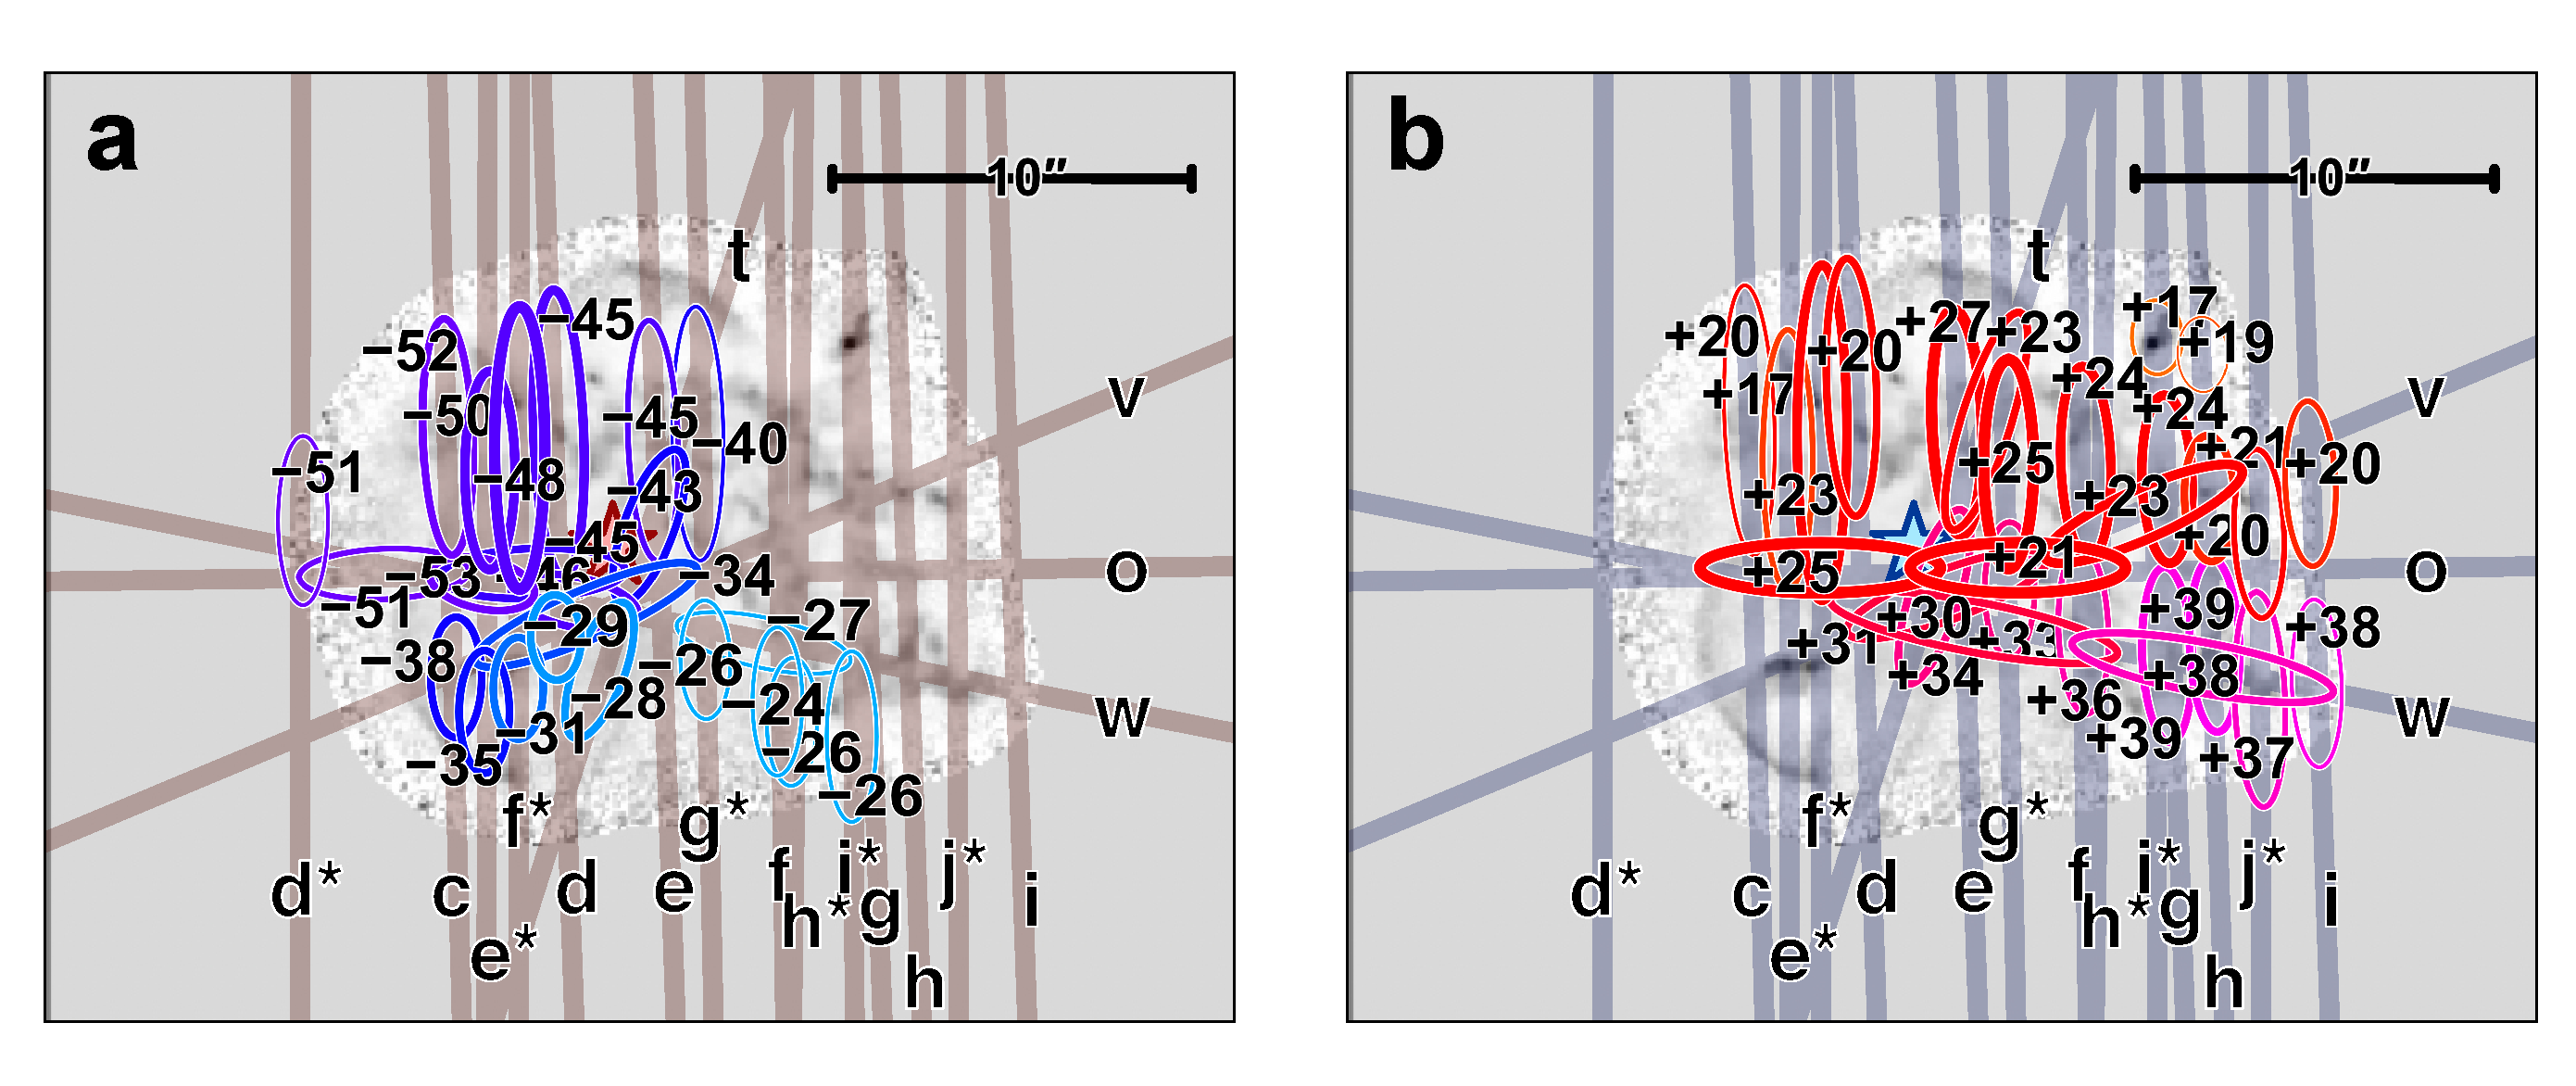
\includegraphics[width=\linewidth]{turtle-knot-complex-map}
  \caption{
    Velocity features in the low-ionization knot complexes,
    which have been identified in the \nii{} slits.
    Left panel shows blue-shifted features,
    while right panel shows red-shifted features,
    each labelled with their line-of-sight velocity
    with respect to the nominal systemic velocity of \SI{40}{km.s^{-1}}.
    The line width is a qualitative indicator of the brightness of each feature.
  }
  \label{fig:knot-complex-map}
\end{figure*}

\begin{figure*}
  \centering
  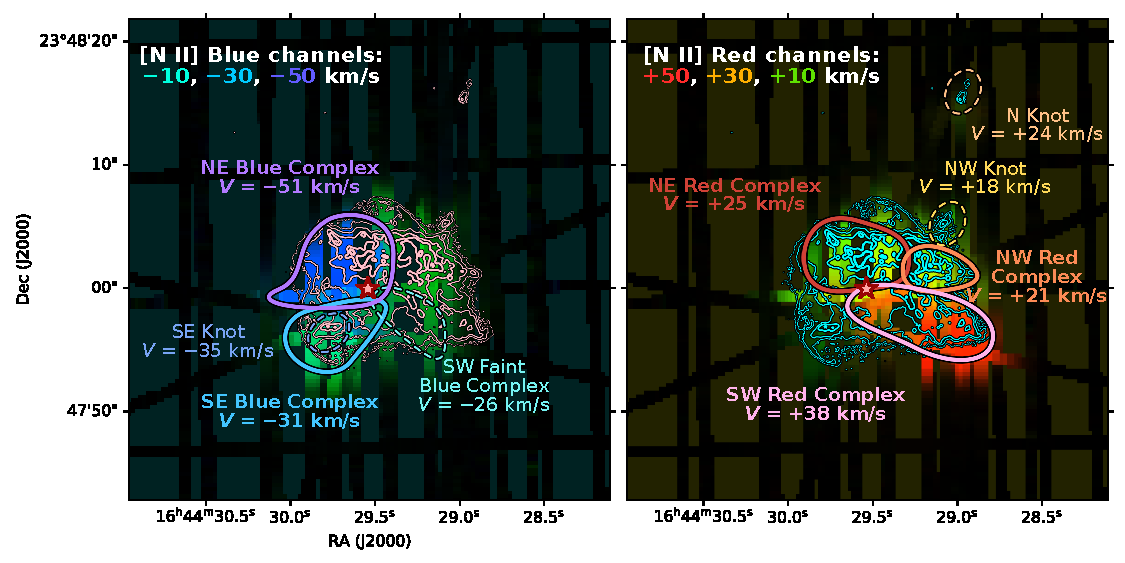
\includegraphics[width=\linewidth]{turtle-nii-knot-complexes}
  \caption{
    Reconstructed velocity channel maps from the \nii{} slit spectra,
    showing the red-shifted (left panel) and blue-shifted (right panel) knot complexes.
    Note that channel maps have not been spatially interpolated,
    so that the individual slit positions can be seen.
    Each color image is constructed from 3 channels, each of width \SI{20}{km.s^{-1}},
    as indicated on the figure.
    All velocities are with respect to the nominal heliocentric systemic velocity of \SI{-40}{km.s^{-1}}.
    The low-ionization emission components from Fig.~\ref{fig:knot-complex-map}
    have been classified into 5 knot complexes,
    which are shown as colored outlines. 
  }
  \label{fig:knot-complexes}
\end{figure*}

\begin{figure}
  \centering
  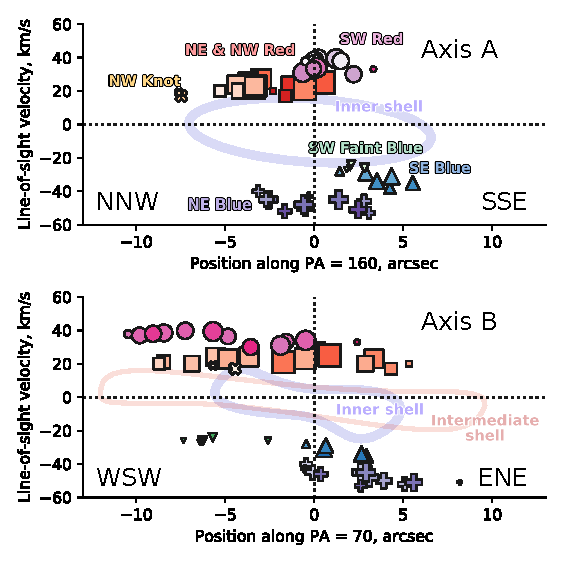
\includegraphics[width=\linewidth]{turtle-knot-complexes-velocity-axes-annotated}
  \caption{
    Radial velocity versus position
    for the low-ionization features features shown in Fig.~\ref{fig:knot-complex-map}.
    Results are shown projected along along the same two axes,
    Axis~A (upper panel) and Axis~B (lower panel),
    as in Fig.~\ref{fig:shell-velocity-axes},
    but this time each feature is shown projected along both axes.
    The features are divided into different knot complexes,
    as shown in Fig.~\ref{fig:knot-complexes},
    which are indicated by symbol type and color.
    Symbol size is proportional to feature brightness (log scale)
    and symbol shade indicates position along the other axis (darker is more positive).
    Continuous lines show the same high ionization shells
    as in Fig.~\ref{fig:shell-velocity-axes}.
  }
  \label{fig:knot-complex-velocity-axes}
\end{figure}

The \nii{} emission from the nebula is dominated by small-scale knots,
as can be appreciated on the \textit{HST} images (Figure~XXX).
These knots have typical sizes \(< 1''\) and so are not spatially resolved
in our ground-based spectroscopy.
A small number of isolated knots are individually detected in our spectra,
but in general we detect only the combined emission of extended knot complexes.
Figure~\ref{fig:knot-complex-map} shows all the \nii{} emission components
identified from our spectra, but excluding those associated with the high-ionization
shells discussed above.
As previously, the components are divided into negative (left panel)
and positive (right panel) velocities.  
In Figure~\ref{fig:knot-complex-velocity-axes}
we classify the emission components into five knot complexes,
plus three individual knots, whose plane-of-sky distribution
and typical line-of-sight velocity are shown
superimposed on the \textit{HST} \nii{} image (contours)
and isovelocity channel maps reconstructed from our slit spectra (color images).

Figure~\ref{fig:knot-complexes} shows the velocity of each \nii{} component
as a function of position along the two axes that characterize the high-ionization shells:
axis~A at \(\text{PA} = \ang{160}\)
and axis~B at \(\text{PA} = \ang{70}\) (see \S~\ref{sec:high-ioniz-shells}).
The kinematics of the shells themselves are shown by faint continuous lines for comparison.
Note that the extent of the velocity axis in this figure
is twice as large as in Figure~\ref{fig:shell-velocity-axes}. 

The clearest axial alignment is seen for the SW Red complex,
which is very tightly clustered around the negative arm of axis~B.
The same is seen to a lesser extent for the NE Blue complex
around the positive arm of axis~B,
but the distribution around the axis is broader in this case.
The remaining complexes have no clear alignment with either axis,
except that the SE Blue complex is marginally more elongated
along the positive arm of axis~A.

The upper panel of Figure~\ref{fig:knot-complex-velocity-axes} indicates
that there is no clear velocity gradient along axis~A,
but the low-ionization knots have significantly faster radial velocities
than the high-ionization shells, by roughly a factor of two.
In addition, there is an asymmetry between the blue and red components:
the blue-shifted knot complexes tend to have a larger radial velocity magnitude,
but to have fainter \nii{} emission, as compared with the red-shifted knot complexes.

From the lower panel of Figure~\ref{fig:knot-complex-velocity-axes},
it is apparent that there is a significant gradient of \(\approx \SI{20}{km.s^{-1}}\)
along axis~B, which is seen in both blue-shifted and red-shifted components.
The sense of this gradient is the same as that seen in the high-ionization shells
along this axis.
It is mainly due to velocity differences
\emph{between} complexes rather than within them,
although both the SW Red and NE Blue complexes
show significant internal gradients of \(\approx \SI{10}{km.s^{-1}}\) in the same direction.

There is an approximate kinematic and spatial symmetry
between pairs of opposite knot complexes:
SW Red with NE Blue complex, and N Red with SE Blue.
It is possible that the west and east sides of the N Red complex
are actually two separate complexes,
in which case the east side would pair with the SW Faint Blue complex,
which would further reinforce this symmetry.

\subsection{Outer lobes}
\label{sec:outer-lobes}

\begin{figure*}
  \centering
  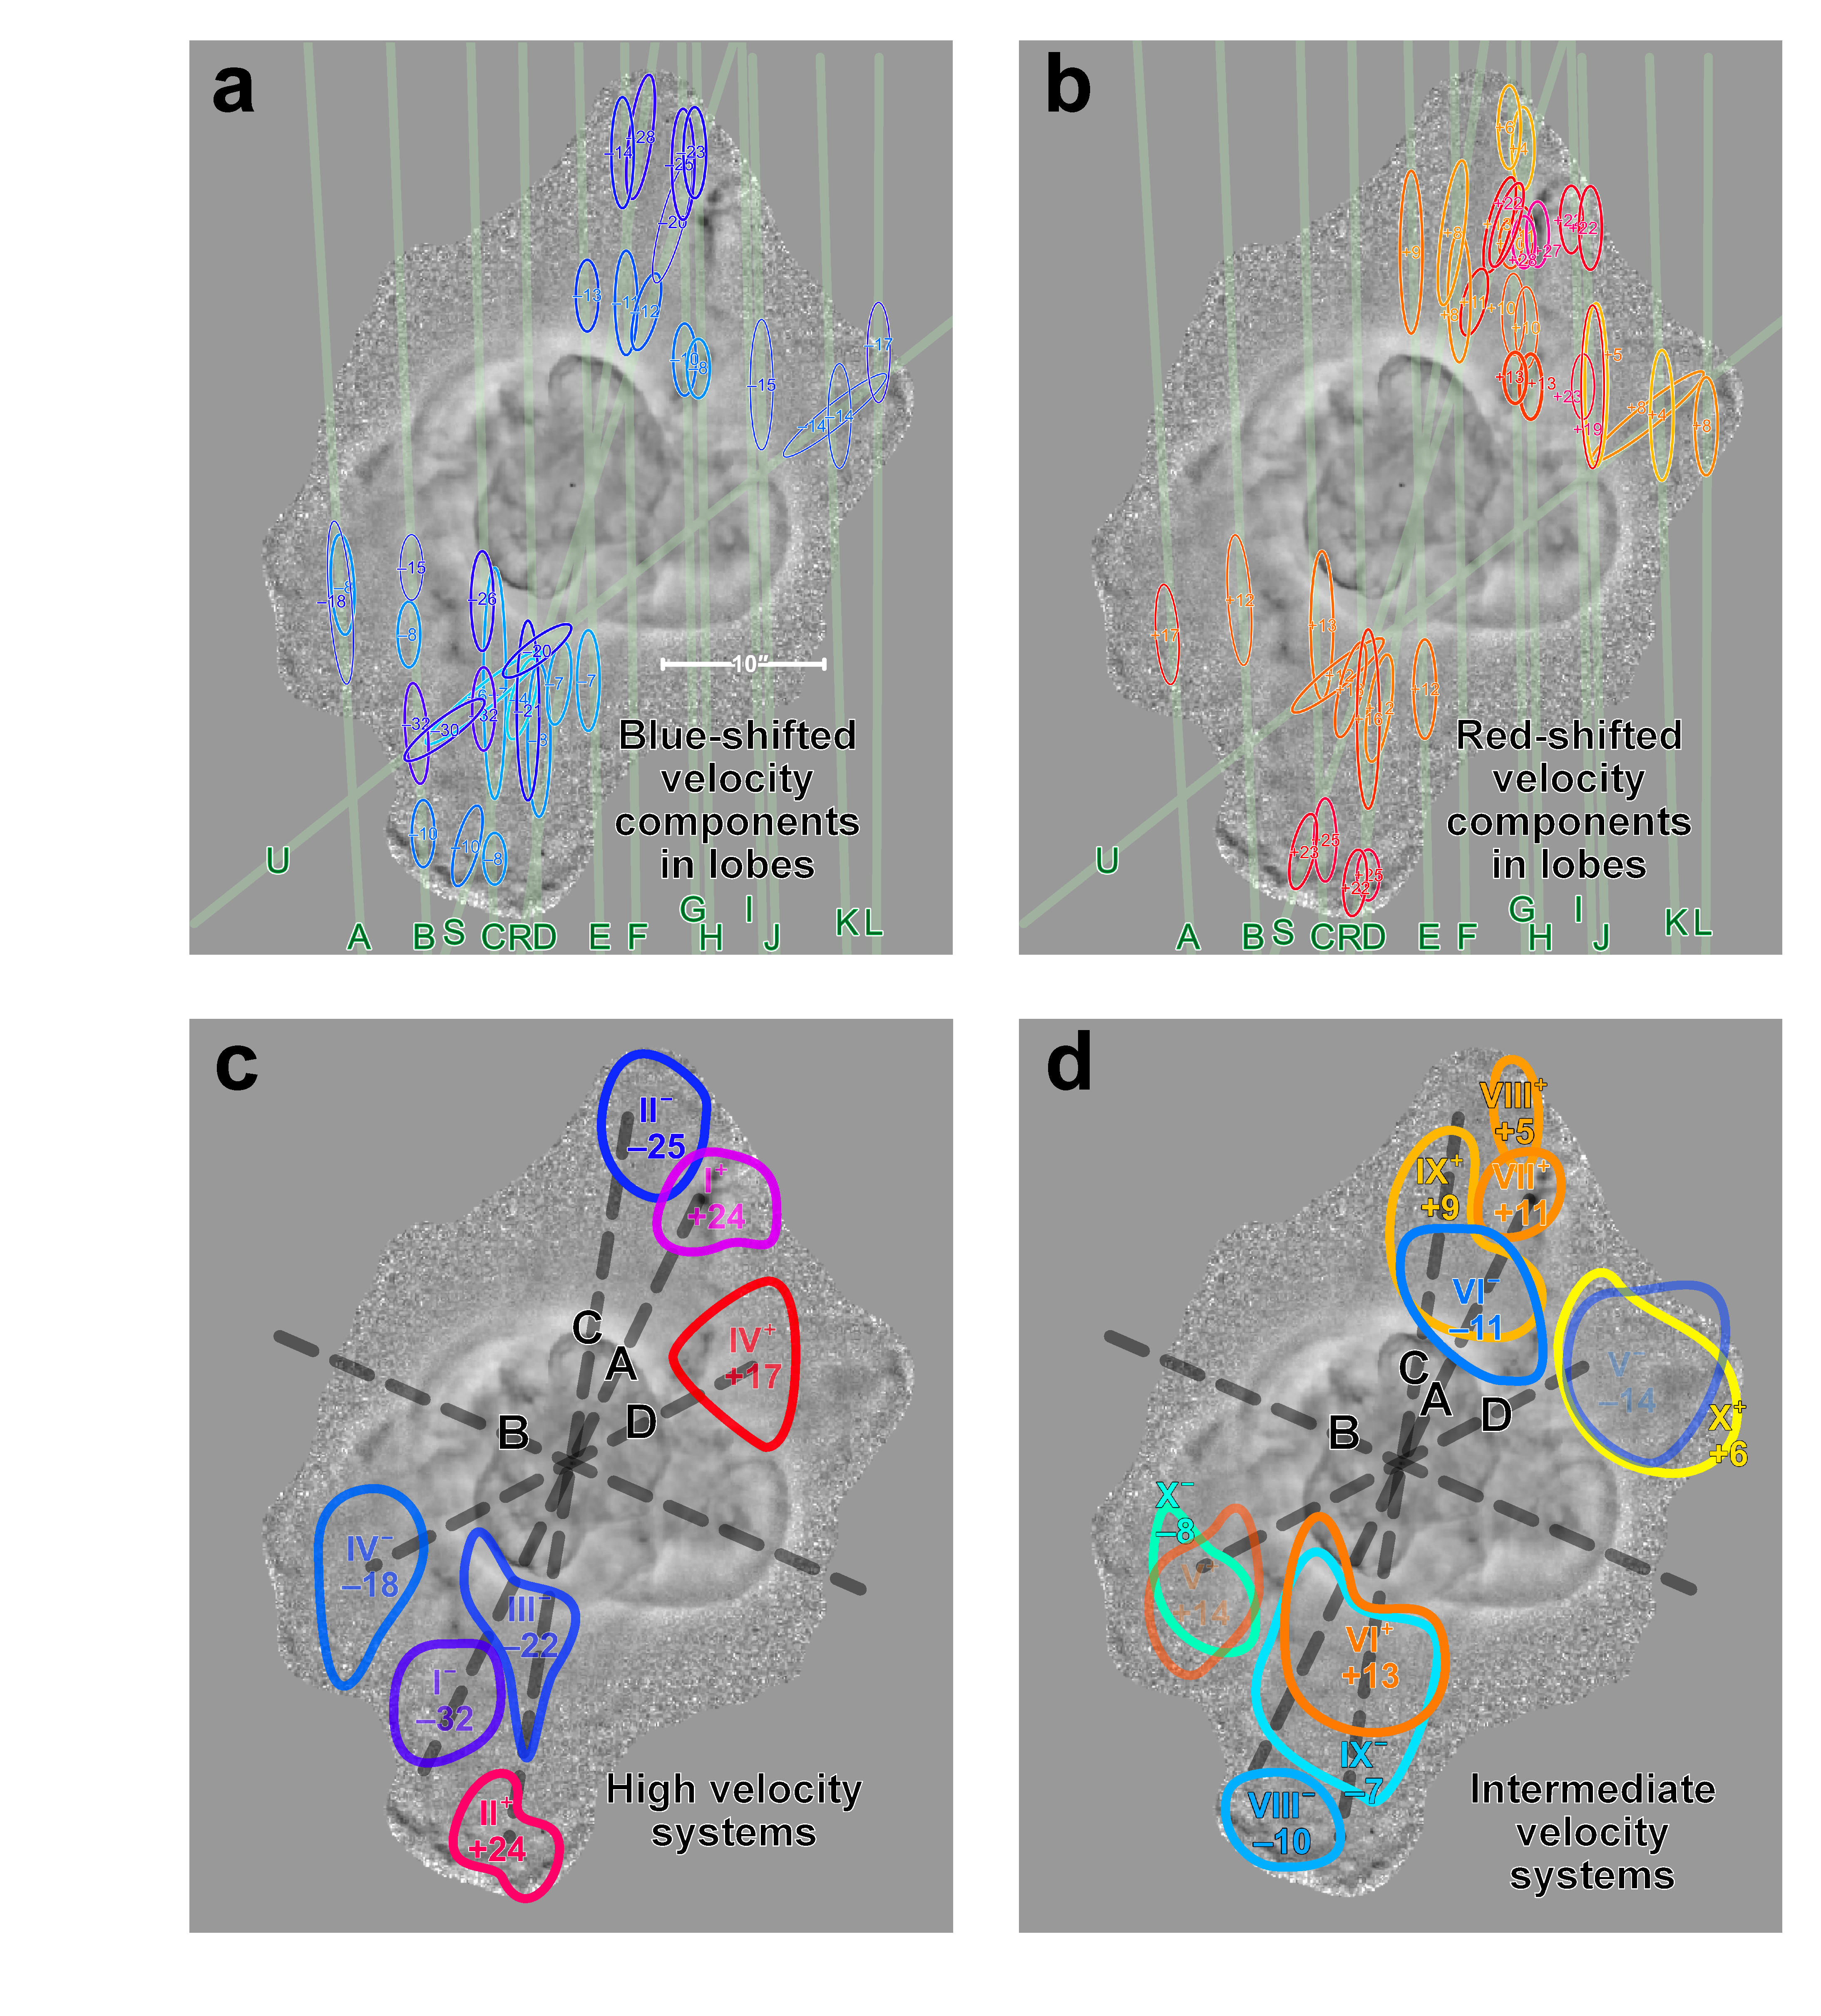
\includegraphics[width=\linewidth]{turtle-lobes-simplified}
  \caption{Velocity components and systems in the outer lobes.}
  \label{fig:outer-lobe-components}
\end{figure*}

\subsection{Haloes}
\label{sec:haloes}

\section{Discussion}
\label{sec:discussion}

\subsection{Velocities and positions in three dimensions}
\label{sec:veloc-posit-three}

Combine radial velocities with proper motions.

\begin{figure}
  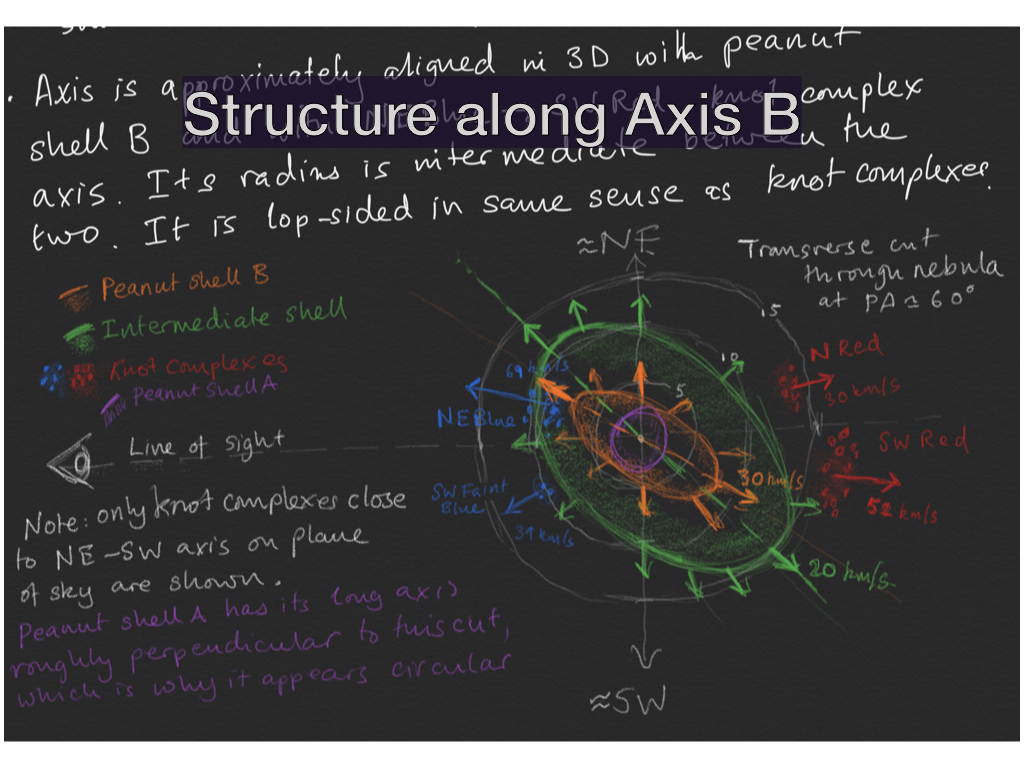
\includegraphics[width=\linewidth]
  {../talk/turtle-talk-morelia-2020-02-export/turtle-talk-morelia-2020-02-export-011}
  \caption{Place-holder figure for three-dimensional reconstruction}
  \label{fig:axis-B-3d}
\end{figure}

\subsection{Flow axes}
\label{sec:flow-axes}

\begin{figure}
  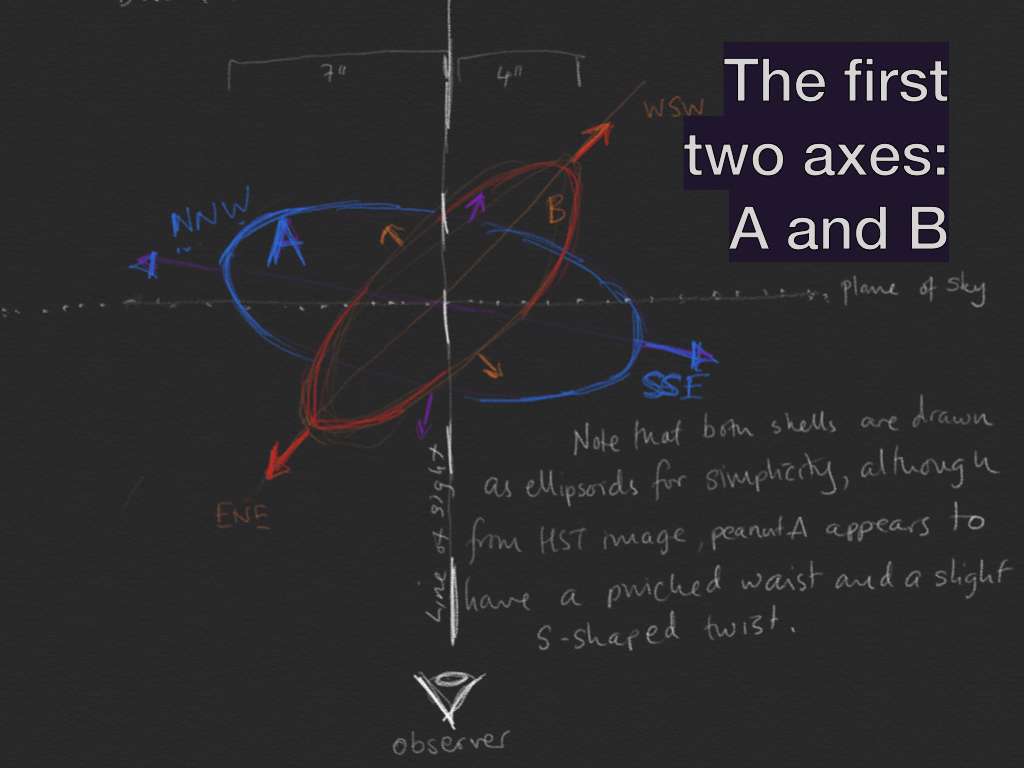
\includegraphics[width=\linewidth]
  {../talk/turtle-talk-morelia-2020-02-export/turtle-talk-morelia-2020-02-export-010}
  \caption{Place-holder figure for Axis A and B}
  \label{fig:flow-axes-AB}
\end{figure}

\begin{figure}
  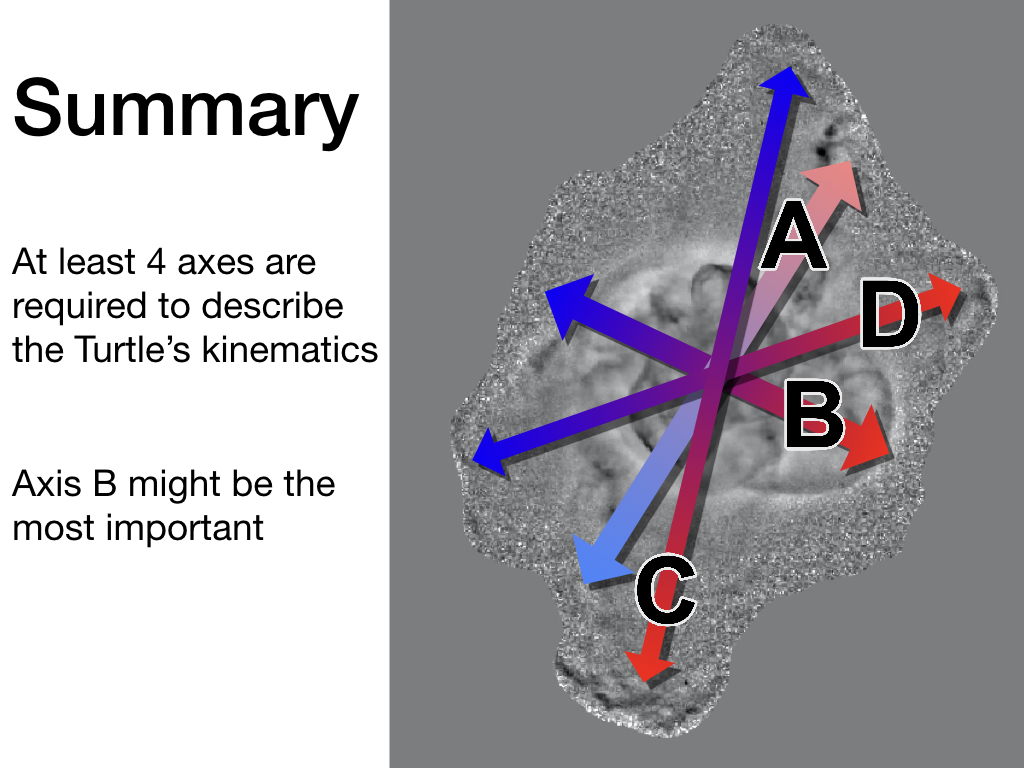
\includegraphics[width=\linewidth]
  {../talk/turtle-talk-morelia-2020-02-export/turtle-talk-morelia-2020-02-export-014}
  \caption{Place-holder figure for all four axes.}
  \label{fig:flow-axes-ABCD}
\end{figure}

\subsection{Dynamical ages}
\label{sec:dynamical-ages}

\begin{figure}
  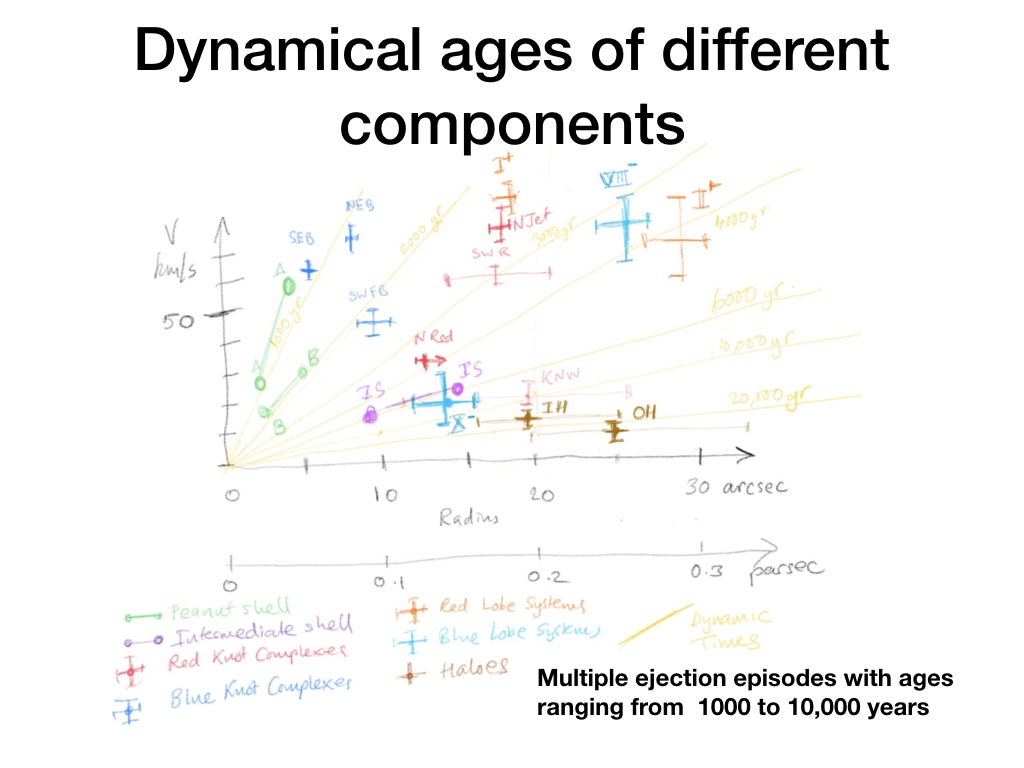
\includegraphics[width=\linewidth]
  {../talk/turtle-talk-morelia-2020-02-export/turtle-talk-morelia-2020-02-export-013}
  \caption{Place-holder figure for dynamical ages}
  \label{fig:ages}
\end{figure}

\bibliography{turtle-refs-will}

% Don't change these lines
\bsp	% typesetting comment
\label{lastpage}

\end{document}


%%% Local Variables:
%%% mode: latex
%%% TeX-master: t
%%% End:
